%%%% ijcai20.tex

\typeout{IJCAI--PRICAI--20 Instructions for Authors}

% These are the instructions for authors for IJCAI-20.

\documentclass{article}
\pdfpagewidth=8.5in
\pdfpageheight=11in
% The file ijcai20.sty is NOT the same than previous years'
\usepackage{ijcai20}

% Use the postscript times font!
\usepackage{times}
\usepackage{soul}
\usepackage{url}
\usepackage[hidelinks]{hyperref}
\usepackage[utf8]{inputenc}
\usepackage[small]{caption}
\usepackage{graphicx}
\usepackage{amsmath}
\usepackage{amsthm}
\usepackage{amssymb}
\usepackage{mathrsfs}
\usepackage{booktabs}
\usepackage{algorithm}
\usepackage{algorithmic}
\usepackage{cleveref}
\urlstyle{same}

% the following package is optional:
%\usepackage{latexsym} 

% See https://www.overleaf.com/learn/latex/theorems_and_proofs
% for a nice explanation of how to define new theorems, but keep
% in mind that the amsthm package is already included in this
% template and that you must *not* alter the styling.
\newtheorem{example}{Example}
\newtheorem{theorem}{Theorem}
\newtheorem{definition}{Definition}
\newtheorem{proposition}{Proposition}
\newtheorem{corollary}{Corollary}

\newcommand{\IE}{\textit{i.e.}}
\newcommand{\EG}{\textit{e.g.}}
\newcommand{\ET}{\textit{et al.}}
\newcommand{\ST}{\textit{s.t.}}


\newcommand{\dd}{\mathrm{d}}
\newcommand{\vv}[1]{\bm{\mathrm{{#1}}}}
\newcommand{\E}{\operatorname{\mathbb{E}}}
\newcommand{\EE}[1]{\operatorname{\mathbb{E}}\left[{#1}\right]}
\newcommand{\EEE}[2]{\operatorname{\mathbb{E}}_{{#1}}\left[{#2}\right]}
\newcommand{\KLD}{\operatorname{KL}}
\newcommand{\KLDD}[2]{\operatorname{KL}\left[{#1}\,\big\|\,{#2}\right]}
\newcommand{\abs}[1]{\left|#1\right|}
\newcommand{\Entropy}{\operatorname{H}}
\newcommand{\Entropyy}[1]{\operatorname{H}\left[#1\right]}
% Following comment is from ijcai97-submit.tex:
% The preparation of these files was supported by Schlumberger Palo Alto
% Research, AT\&T Bell Laboratories, and Morgan Kaufmann Publishers.
% Shirley Jowell, of Morgan Kaufmann Publishers, and Peter F.
% Patel-Schneider, of AT\&T Bell Laboratories collaborated on their
% preparation.

% These instructions can be modified and used in other conferences as long
% as credit to the authors and supporting agencies is retained, this notice
% is not changed, and further modification or reuse is not restricted.
% Neither Shirley Jowell nor Peter F. Patel-Schneider can be listed as
% contacts for providing assistance without their prior permission.

% To use for other conferences, change references to files and the
% conference appropriate and use other authors, contacts, publishers, and
% organizations.
% Also change the deadline and address for returning papers and the length and
% page charge instructions.
% Put where the files are available in the appropriate places.

\title{VAEPP: Variational Autoencoder with a Pull-back Prior}

% Single author syntax
%\author{
%    Christian Bessiere
%    \affiliations
%    CNRS, University of Montpellier, France
%    \emails
%    pcchair@ijcai20.org
%}

% Multiple author syntax (remove the single-author syntax above and the \iffalse ... \fi here)
% Check the ijcai20-multiauthor.tex file for detailed instructions
\author{
}

\begin{document}

\maketitle


\pagestyle{plain}


\begin{abstract}
  The {\it IJCAI--PRICAI--20 Proceedings} will be printed from electronic
  manuscripts submitted by the authors. The electronic manuscript will
  also be included in the online version of the proceedings. This paper
  provides the style instructions.
\end{abstract}

\section{Introduction}

How to learn deep generative models that are able to capture complex data pattern in high dimension space, \EG image datasets, is one of the major challenges in machine learning. Many approaches to training generative models by distinct training objectives have been proposed in the past, \EG Generative Adversarial Networks (GAN)~\cite{goodfellow2014generative}, Flow-based models~\cite{dinh2016density,kingma2018glow}, PixelCNN~\cite{van2016conditional}, and Variational Autoencoders (VAE)~\cite{kingma2014auto,rezende_stochastic_2014}.

VAE uses the variational inference and re-parameterization trick to optimize the evidence lower bound of log-likelihood (ELBO). In the past, many researches~\cite{kingma2016improved,tomczak2016improving} focused on enriching the variational posterior, but recently \cite{tomczak2018vae} showed that the standard Gaussian prior could lead to underfitting in latent space, harmful to the performance of VAEs. To enrich the prior, several learnable priors have been proposed~\cite{tomczak2018vae,bauer2019resampled,takahashi2019variational}. Most of them focus on approximating aggregated posterior which is the integral of the variational posterior and is shown as the optimal prior to minimize ELBO. However, existing methods based on the aggregated posterior reach limited performance, and the practical meaning of the aggregated posterior is blurry. Recently, we notice that the discriminator can assess the quality of data and \textbf{we argue that it is advisable to adjust the learnable prior by a discriminator which has clearer practical meaning than approximating the aggregated posterior. } 

We propose Pull-back Prior, based on the discriminator and a learnable prior. 
Firstly, a discriminator $D(x)$ is trained for assessing the quality of images. Then, we define a pull-back discriminator on latent space, by $D(G(z))$, where $G(z)$ is the generator (notion \textit{pull-back} is from mathematics). Finally, we adjust the density of the prior according to the pull-back discriminator. 
%The inference of pull-back prior is similar to the proof that shows aggregated posterior as optimal prior. 
%The key difference is that we search the prior that minimizes the Wasserstein distance between empirical distribution and model distribution instead of ELBO (if so, we will obtain aggregated posterior). 

We propose a training algorithm for VAE with Pull-back Prior (VAEPP), based on SGVB~\cite{kingma2014auto} with gradient penalty terms, which mix the discriminator and the gradient penalty term into VAE. We extend it to a more general VAE framework. We also use Langevin Dynamics to improve the quality of sampling. 
Thanks to the gradient penalty term of WGAN-GP~\cite{gulrajani2017improved} and WGAN-div~\cite{wu2018wasserstein}, and the practical implementation of Langevin dynamics in MEG~\cite{kumar2019maximum}, we enjoy stable efficient training and sampling process. 
% In these years, out-of-distribution (OoD) is noticed by some researchers, and \cite{nalisnick2018deep} has shown that the model log-likelihood from flow-based models, VAEs, and PixelCNN assign higher density to the images of SVHN~\cite{netzer2011reading} when these models are trained on CIFAR-10 and such peculiar behavior of these models also act on other dataset. It challenges the assumption of generative models that the density of in-distribution is higher and the density of out-of-distribution is lower. In this paper, we will show that the discriminator and the norm of its gradient are as our expectation in VAEPP. It reminds us to use these indicators to help VAE to outcome the OoD problem, and it reaches a powerful performance in OoD testing.

The main contributions of this paper are in the following:
\begin{itemize}
	\item We propose a novel and powerful learnable prior, Pull-back Prior, which is adjusted by a discriminator that can assess the quality of data. 
	\item We propose VAEPP framework to use existing techniques of VAE, \EG flow posterior, and WGAN, \EG gradient penalty strategy, and Langevin Dynamics to improve the log-likelihood, quality of sampling and stability of training. 
	\item In MNIST and CIFAR-10, the log-likelihood of VAEPP outperforms models without autoregressive components and is comparable to autoregressive models. In MNIST, Fashion-MNIST, CIFAR-10 and CelebA,  the FID of VAEPP is comparable to GANs and SOTA of VAE. 
	% \item The combination indicator of VAEPP which involves the log-likelihood and discriminator outperforms other existing OoD detector in OoD testing.
\end{itemize}

\section{Background}

\section{Pull-back Prior}\label{sec:pull_back_prior}

\subsection{Intuition of Pull-back Prior}\label{subsec:intuition}

The formula of Pull-back Prior is given by:
\begin{equation}\label{eq:pull_back_prior}
	p_\lambda(z) = \frac{1}{Z} p_\mathcal{N}(z) \cdot e^{- \beta D(G(z))} \tag{4}
\end{equation}
where $p_\mathcal{N}$ is a simple prior, $D$ is a discriminator, $G$ is the generator $G(z) = \E_{p_\theta(x|z)} x$, $Z$ is the partition function $Z = \int_{\mathcal{Z}} p_\mathcal{N}(z) \exp\{- \beta * D(G(z))\} \dd z$ and $\beta$ is a learnable scalar.

An intuitive explanation of Pull-back Prior is that we improve the density of $z$ which generates better data and decrease the density of $z$ which generates worse data. 
$D$ is a discriminator to assess the quality of $x$. When $D(x)$ is less, $x$ is more similar to real data and vice versa, as shown in \cref{fig:interpolate}. The pull-back discriminator is defined by $D(G(z))$, representing the quality of the data generated by $z$. To improve the density at the better $z$ and decrease the density at the worse $z$, we modify $p_\mathcal{N}(z)$ by $\beta D(G(z))$ and then normalize it by $Z$. 

We obtain the basic formula of Pull-back Prior, and $p_\mathcal{N}$ is a special case where $\beta = 0$. The theoretical derivation for Pull-back Prior is provided in \cref{subsec:inference}. However, it remains questions about how to obtain $D$ and $G$, determine $\beta$, and calculate $Z$. 

\begin{figure}[tb]
	\centering
	
\includegraphics[width=0.9\columnwidth]{../figures/interpolate}
	\caption{
	The discriminators on above images (generated by linear interpolation of two sample from $q_\phi(z)$), are better at both sides and worse at the middle, which validates the intuition that a discriminator can assess the quality of images. Moreover, the density of $z$ which generates better images will increase, and the density of $z$ which generates worse images will decrease. 
%2825-plot_samples mean and std is 9.528099, 0.0050279954
%[array([[9.547822]], dtype=float32), array([[9.583102]], dtype=float32), array([[9.603901]], dtype=float32), array([[9.626318]], dtype=float32), array([[9.633714]], dtype=float32), array([[9.632847]], dtype=float32), array([[9.631333]], dtype=float32), array([[9.640044]], dtype=float32), array([[9.631817]], dtype=float32), array([[9.654361]], dtype=float32), array([[9.641564]], dtype=float32), array([[9.600273]], dtype=float32), array([[9.559095]], dtype=float32), array([[9.533435]], dtype=float32), array([[9.468535]], dtype=float32)]
%Normalized is [  3.92263684,  10.93934971,  15.07598834,  19.53442519,
%        21.00538915,  20.83295462,  20.53184058,  22.26434018,
%        20.62810161,  25.11179704,  22.56664754,  14.35442841,
%         6.16468344,   1.06125793, -11.84647066]
	}
	\label{fig:interpolate}
\end{figure}

\subsection{How to obtain $D$ and $G$}\label{subsec:determine_D_and_G}
By definition in \cref{eq:pull_back_prior}, $G$ is defined, and in practical networks, it is generated by neural network and $p_\theta(x|z)$ set it as mean (\EG $p_\theta(x|z)$ is Gaussian or Bernouli). 

$D$ plays an important role in Pull-back Prior. We propose two way to obtain $D$ and compare their difference detaily in \cref{subsec:improve_of_vaepp} and \cref{subsec:naive_vaepp}. 

\subsection{How to determine $\beta$}\label{subsec:determine_beta}

Theoretically, $\beta$ in \cref{eq:pull_back_prior} represents how far $p_\lambda$ is from $p_\mathcal{N}$, as proved in \cref{subsec:inference}.
%but how to decide the value of $\beta$? When $\beta$ is smaller, the difference between $p_\lambda$ and $p_\mathcal{N}$ is less, \IE the influence of discriminator is severely limited. When $\beta$ is larger, $p_\lambda$ is farther from $p_\mathcal{N}$. Noticing that in \cref{eq:final_optimization}, we simplify the optimization of $D$ by an approximated $D$, if $p_\lambda$ is too far from $p_\mathcal{N}$, this approximation will become invalid. 
%Consequently, $\beta$ should be set to an appropriate value which can't severely limit the influence of discriminator and could ensure that approximated $D$ is valid. 
It is important to realize that the Pull-back Prior is serving for better ELBO. 
%Whatever the function family of $p_\lambda$ is limited or approximation $D$ is invalid, the ELBO will suffer. 
Therefore, it is reasonable to search $\beta$ by the optimization for ELBO ($\lambda$ contains $\beta$ and $\omega$, which is the parameters of $D$):
\begin{equation}
	\beta = \arg \min_{\beta} \mathcal{L}(\theta, \phi, \lambda) = \arg \min_{\beta} \mathcal{L}(\theta, \phi, \beta, \omega) \tag{5}
\end{equation}
The optimization process of $\beta$ depends on $\partial \mathcal{L}/\partial \beta$:
\begin{align*}\label{eq:behavior_of_beta}
\frac{\partial \ln Z}{\partial \beta} &= \frac{1}{Z} \int p_\mathcal{N}(z) e^{-\beta D(G(z))} \cdot (-D(G(z))) \dd z \\
&=  \E_{p_\lambda(z)} - D(G(z))  \\
\frac{\partial \mathcal{L}}{\partial \beta} &= \E_{q_\phi(z)}[ -D(G(z))] - \frac{\partial \ln Z}{\partial \beta} \\
&= - \E_{q_\phi(z)}[ D(G(z))] + \E_{p_\lambda(z)}[ D(G(z))]   \tag{6}
\end{align*}
The 1st term in \cref{eq:behavior_of_beta} is the mean of the discriminator on the reconstructed data, which is nearly same as real data when the reconstruction is well-trained. The 2nd term in \cref{eq:behavior_of_beta} is the mean of the discriminator on data generated from $p_\lambda$. Hence, $\partial \mathcal{L}/\partial \beta = 0$ means that the discriminator can't distinguish the reconstructed data and generated data, which coincides with the philosophy of GANs.

\subsection{The lower bound of $Z$}\label{subsec:determine_z}

The extract calculation of partition function $Z$ is difficult. But in VAE domain, it is acceptable to obtain a lower-bound of log-likelihood. Therefore, we propose a feasible evaluation for upper-bound of $Z$, called $\hat{Z}$, which will not over-estimate log-likelihood. 
It is given by:
\begin{align*}\label{eq:Z_estimator}
	Z = \E_{q_\phi(z)}\frac{f_\lambda(z)}{q_\phi(z)} \leq \E_{q_\phi(z)} \frac{f_\lambda(z)}{\hat{q}_\phi(z)} = \hat{Z} \tag{8}
\end{align*}
where $f_\lambda(z) = p_\mathcal{N}(z) \exp\{- \beta D(G(z))\}$ and $\hat{q}_\phi(z)$ is a lower-bound of $q_\phi(z)$. It is easy to show that
\begin{align*}
	p_\theta(x) = \int \frac{1}{Z} p_\theta(x|z) f_\lambda(z) \dd z &\geq \int \frac{1}{\hat{Z}} p_\theta(x|z) f_\lambda(z) \dd z \\
\mathcal{K} = \E_{q_\phi(z)} \frac{1}{Z} \ln f_\lambda(z) &\geq \E_{q_\phi(z)} \frac{1}{\hat{Z}}\ln f_\lambda(z) = \mathcal{\hat{K}} \\
\mathcal{L} = \mathcal{I} + \mathcal{J} + \mathcal{K} &\geq \mathcal{I} + \mathcal{J} + \mathcal{\hat{K}} = \mathcal{\hat{L}}
\end{align*}
Above ineqaulities show that, if we replace $Z$ by $\hat{Z}$ we will obtain lower-bound of log-likelihood and ELBO. Such that $\hat{Z}$ could be used in training and evaluation, and it will not over-estimate log-likelihood and ELBO. 

The key of \cref{eq:Z_estimator} is the choice of $\hat{q}_\phi(z)$. As we mentioned before, $q_\phi(z)$ is intractable to compute the exact density, but $q_\phi(z|x)$ is feasible. We introduce a lower-bound of  $q_\phi(z)$:
\begin{equation*}
	q_\phi(z) = \E_{p^*(x)} q_\phi(z|x) \approx \frac{1}{N}\sum_{i=1}^N q_\phi(z|x^{(i)}) \geq \frac{1}{N} q_\phi(z|x^{(j)})
\end{equation*}
where $x^{(j)}$ is a real data, $N$ is the size of training set and RHS is the $\hat{q}_\phi(z)$. To reduce the gap between $\hat{q}_\phi(z)$ and $q_\phi(z)$, $q_\phi(z|x^{(j)})$ should be one of the largest in the summation. Therefore, we firstly sample $x^{(j)}$ form dataset, and then sample $z$ from $q_\phi(z|x^{(j)})$. By this way, $q_\phi(z|x^{(j)})$ is  large enough. 

In MNIST and other Bernouli image datasets, the number of Bernouli images sampled from real images might be numerous and $\hat{q}_\phi(z)$ might be underestimiated. To solve this it, we propose ELBO based on $q_\phi(z|e)$ instead of $q_\phi(z|x)$:
\begin{align*}~\label{eq:another_elbo}
	&\E_{p^*(x)} \ln p_\theta(x) \geq \E_{p^*(e)} \E_{p^*(x|e)} \ln \E_{q_\phi(z|e)} \frac{p_\theta(x|z)p_\theta(z)}{q_\phi(z|e)} \\
	 &= \E_{p^*(e)} \E_{p^*(x|e)} \E_{q_\phi(z|e)} \ln \frac{p_\theta(x|z)p_\theta(z)}{q_\phi(z|e)} \tag{7} \\
	 &= \E_{p^*(x)} \ln p^*(x) - \E_{p^*(e)} \E_{p^*(x|e)} KL(q_\phi(z|e), p_\theta(z|x))
\end{align*} 
where $p^*(x)$ is sampled from $p^*(e)$, and $p^*(x|e)$ means the sampling process from $e$. \cref{eq:another_elbo} is similar to the original ELBO~\cref{eq:ELBO}, and the above conclusion about learnable prior holds for \cref{eq:another_elbo} by repeating above inference. Moreover, the situation without Bernouli images is a special case where $p^*(x|e) = \delta(x - e)$. % Additionally, when $p_\theta(x|z)$ and $p^*(x|e)$ is both Bernouli, term $\E_{p^*(x|e)} \ln p_\theta(x|z)$ has analytical solution $x\log e+(1-x)\log(1-e)$, which could make the training and evaluation more stable (don't need sample $x$). 
Since $q_\phi(z|e)$ is known, $\hat{q}_\phi(z)$ is feasible by $\frac{1}{N} q_\phi(z|e^{(j)})$. 

By the theory of importance sampling, $p_\lambda$ is the optimal choice for the proposal distribution in estimation of $Z$ but it is expensive to sample from $p_\lambda$. 
\cite{bauer2019resampled} uses $p_\mathcal{N}$ as proposal distribution to estimate $Z$ but when $KL(p_\mathcal{N}, p_\lambda)$ is high, the variance of this estimation will be large. In experiment, $KL(q_\phi, p_\lambda)$ is much less than $KL(q_\phi, p_\mathcal{N})$ in trained model. Therefore, we choose $q_\phi(z)$ as proposal distribution and use a feasible $\hat{q}_\phi(z)$ to replace $q_\phi(z)$ in \cref{eq:Z_estimator}. The variance of $\hat{Z}$ is acceptable in experiment.  

In training, $\beta$ is trained from small to large and $KL(p_\mathcal{N}, p_\lambda)$ is so. Therefore, $p_\mathcal{N}$ is also used as proposal distribution in training. 
\section{Training and Sampling}\label{sec:vaepp}
In this section, we will propose two training methods and a sampling method for VAEPP. The main difference between these two trainings method is the training method of the discriminator. 

\subsection{Naive training for VAEPP} \label{subsec:naive_vaepp}
By \cref{subsec:inference}, an approximation discriminator is trained by:
\begin{equation*}
	W^1(p^\dag, p^*) = \sup_{Lip(D) \leq 1} \E_{p^\dag} D(x) - \E_{p^*} D(x)
\end{equation*} 
where $p^\dag(x) = \E_{p_\mathcal{N}(z)} p_\theta(x|z)$. The real discriminator should be obtained by $W^1(p_\theta, p^*)$, but it is expensive to sample from $p_\theta$ in training and $W^1(p^\dag, p^*)$ is used to obtain an approximation discriminator. Therefore, the approximation discriminator may be invalid when $p_\lambda$ is too far from $p_\mathcal{N}$, \IE $\beta$ is too large. Fortunately, the training for $\beta$ can avoid this: when $\beta$ becomes too large and $D$ becomes invalid, ELBO will be worse and then $\beta$ will decrease. The other parameters is trained by SGVB:
\begin{equation*}
	\max_{\theta, \phi, \beta} \mathcal{L}(\theta, \phi, \beta, \omega)
\end{equation*}
Above two training process run alternatively, which is called the naive training algorithm for VAEPP, in \cref{alg:vaepp},. 
\begin{algorithm}[tb]
\caption{The naive training algorithm for VAEPP}
\label{alg:vaepp}
\textbf{Require}: The gradient penalty algorithm $R$, the batch size $b$, the number of critic iterations per generator iteration $n_c$, the parameters for Adam Optimizers, $\tau$. 

\begin{algorithmic}[1] %[1] enables line numbers
\WHILE{$\theta, \phi, \beta, \omega$ have not converged}
\FOR {$k = 1, \ldots n_c$}
\FOR {$i = 1, \ldots, b$}
\STATE Sample $e, x \sim p^*$, $z \sim q_\phi(z|e)$, $\epsilon \sim p_\mathcal{N}$
\STATE $Z^{(i)} \gets \frac{1}{2}(\exp\{-\beta D(G(\epsilon))\} + \frac{f_\lambda(z)}{\hat{q}_\phi(z)})$
\STATE $\mathcal{L}^{(i)} \gets \ln p_\theta(x|z) + \ln f_\lambda(z) - \ln q_\phi(z|e)$
\ENDFOR
\STATE $\mathcal{L} \gets \frac{1}{b}\sum_{i}^b \mathcal{L}^{(i)} - \ln (\frac{1}{b}\sum_{i}^b Z^{(i)})$
\STATE $\theta, \phi, \beta \gets $ Adam $(\nabla_{\theta, \phi, \beta} \mathcal{L}, \{\theta, \phi, \beta\}, \tau)$
\ENDFOR
\FOR {$i = 1, \ldots, b$}
\STATE Sample $e, x \sim p^*$, latent variable $z \sim p_\mathcal{N}$
\STATE	$\hat{e} = G(z)$, get gradient penalty $\zeta \gets R(e, \hat{e})$
\STATE $L^{(i)} \gets D(\hat{x}) - D(x) + \zeta$
\ENDFOR
\STATE $\omega \gets $ Adam $(\nabla_{\omega} \frac{1}{b}\sum_{i}^b L^{(i)}, \omega, \tau)$
\ENDWHILE
\end{algorithmic}
\end{algorithm}

\subsection{Combing training for VAEPP} \label{subsec:improve_of_vaepp}

\begin{figure}[tb]
	\centering
	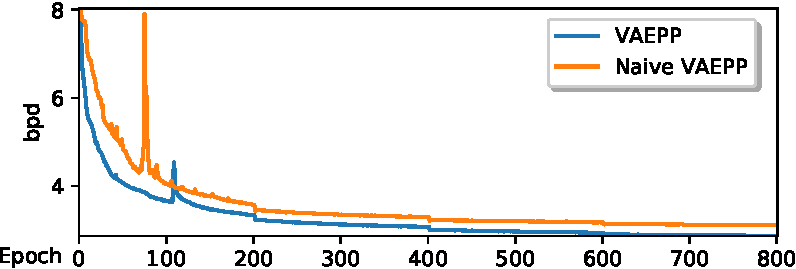
\includegraphics[width=0.9\columnwidth]{../dist.strip/loss_curves}
	\caption{
	Training process of Naive VAEPP and VAEPP on CIFAR-10. Naive VAEPP is more unstable and nearly crashes at 80 epoch while VAEPP has a little acceptable gap. From global view, the training loss of VAEPP is more smooth than Naive VAEPP and is better than Naive VAEPP over almost all training process, which validates the motivation in \cref{subsec:improve_of_vaepp}. There are little gaps at per 200 epoch because learning rate is reduced to half at every 200 epoch. 
	}
	\label{fig:loss_curves}
\end{figure}

However, the training process of \cref{alg:vaepp} is unstable and inefficient, as shown in \cref{fig:loss_curves}. 
We suspect that the two independent optimization instead of one whole optimization, may lower the log-likelihood and stability. Therefore, we try to combine the training for $\theta, \phi, \beta, \omega$ into a whole optimization. 
Our solution is to use SGVB with gradient penalty regularizer to train VAEPP:
\begin{equation*}
	\max_{\theta, \phi, \beta} \max_{Lip(D) \leq 1} \mathcal{L}(\theta, \phi, \beta, \omega) 
\end{equation*} 
In such optimization, the behavior of $\theta, \phi, \beta$ is same as \cref{alg:vaepp} since the optimization for them is same. For $\omega$, 
$\max_{Lip(D) \leq 1} \mathcal{L}(\theta, \phi, \beta, \omega)$ indeed finds a suboptimal discriminator in $W^1(p^\dag, p^*)$ (sign $\simeq$ means that optimizations at left and right are equivalent):
\begin{align*}\label{eq:improve_vaepp}
	&\max_{Lip(D) \leq 1} \mathcal{L} \simeq \max_{Lip(D) \leq 1} \{ -\E_{q_\phi(z)} \beta*D(G(z)) - \ln Z \}\\ 
	&\leq \beta \max_{Lip(D) \leq 1} \{ \E_{p_\mathcal{N}(z)} D(G(z)) - E_{q_\phi(z)} D(G(z)) \} \tag{9} \\
	&= \beta W^1(p^\dag, p_r) \approx \beta W^1(p^\dag, p^*) 
\end{align*}
where $p_r$ denotes $p_r(x) = \E_{q_\phi(z)} p_\theta(x|z)$, consisting of reconstructed data. 
The last approximation sign is from the fact that $p_r \rightarrow p^*$ after a few epoch in training of VAE. \cref{eq:improve_vaepp} also uses the assumption $D(G(z)) = \E_{p_\theta(x|z)} D(x)$ introduced in \cref{subsec:inference} to simplify equation. The inequality of $\ln Z$ is in the following:
\begin{equation*}
	\ln Z = \ln \E_{p_\mathcal{N}(z)} e^{- \beta * D(G(z))} \geq \E_{p_\mathcal{N}(z)} [- \beta * D(G(z))]
\end{equation*}

\cref{eq:improve_vaepp} indicates that it is reasonable to obtain a suboptimal discriminator $D$ by optimizing $\mathcal{L}$ with the gradient penalty term, and the gradient penalty term should be multiplied by $\beta$. In this way, the optimizations for $\theta, \phi, \beta$ and $\omega$ are combined into one, which is provided in \cref{alg:improved_vaepp}. 
Thanks to the gradient penalty regularizer term provided by WGAN-GP and WGAN-div, we enjoy stable and efficient training. The model trained by \cref{alg:vaepp} is called Naive VAEPP and the model trained by \cref{alg:improved_vaepp} is called VAEPP. 
\begin{algorithm}[tb]
\caption{The combing training algorithm for VAEPP}
\label{alg:improved_vaepp}
\textbf{Require}: The gradient penalty algorithm $R$, the batch size $b$, the parameters for Adam Optimizers, $\tau$. 

\begin{algorithmic}[1] %[1] enables line numbers
\WHILE{$\theta, \phi, \beta, \omega$ have not converged}
\FOR {$i = 1, \ldots, b$}
\STATE Sample $e, x \sim p^*$, $z \sim q_\phi(z|e)$, $\epsilon \sim p_\mathcal{N}$
\STATE $\hat{e} = G(\epsilon)$, get gradient penalty $\zeta \gets R(e, \hat{e})$ 
\STATE $Z^{(i)} \gets \frac{1}{2}(\exp\{-\beta D(G(\epsilon))\} + \frac{f_\lambda(z)}{\hat{q}_\phi(z)})$
\STATE $\mathcal{L}^{(i)} \gets \ln p_\theta(x|z) + \ln f_\lambda(z) - \ln q_\phi(z|e) + \beta \zeta$
\ENDFOR
\STATE $\mathcal{L} \gets \frac{1}{b}\sum_{i}^b \mathcal{L}^{(i)} - \ln (\frac{1}{b}\sum_{i}^b Z^{(i)})$
\STATE $\theta, \phi, \beta, \omega \gets $ Adam $(\nabla_{\theta, \phi, \beta} \mathcal{L}, \{\theta, \phi, \beta, \omega\}, \tau)$
\ENDWHILE
\end{algorithmic}
\end{algorithm}

\subsection{Sampling from VAEPP}
We apply Langevin Dynamics to sample $z$ from $p_\lambda(z)$. It could generate natural and sharp images and only requires that $\nabla_z \log p_\lambda(z)$ is computable and the initial $z_0$ has an enough high density in $p_\lambda(z)$~\cite{song2019generative}. 
Moreover, MEG~\cite{kumar2019maximum} have implemented a Metropolis-Adjusted Langevin Algorithm (MALA) for sampling where the formula of density also contains a discriminator term. But how to obtain the initial $z_0$ whose density is high enough is still a problem. 

Following the philosophy of VAEPP, \IE using the technique of GANs to assist VAEs, it is natural to use a GAN to model the distribution $q_\phi(z)$, and use samples of the GAN as the initial $z_0$ for MALA. 

The sampling of VAEPP consists of 3 parts: 
\begin{enumerate}
	\item generate initial $z_0$ by a GAN modeling $q_\phi(z)$
	\item generate $z \sim p_\lambda(z)$ from initial $z_0$ by MALA
	\item generate image from $z$ with a decoder
\end{enumerate}

This sampling process is similar to 2-Stage VAE~\cite{dai2019diagnosing}. The main difference between them is that VAEPP applies Langevin Dynamics to sample from the explicit prior but 2-Stage VAE doesn't, since the prior of 2-Stage VAE is implicit. In experiments, sampling from the explicit learnable prior improves the quality of sampling and ensures the theoretical correctness of the prior. 

It is hard to sample $z$ from $p_\lambda(z)$ since it is complicated. Accept/Reject Sampling (ARS)~\cite{bauer2019resampled} is unuseful for $p_\lambda$ because ARS requires that $p_\lambda(z) / p_\mathcal{N}(z)$ is bounded by a constant $M$, such that a sample could be sampled in $M$ times. It means $\beta$ is nearly 0, but not in fact.
 
 
\section{Experiments}

\subsection{Log-likelihood}


\subsection{Quality of Sampling}


\subsection{Out-of-Distribution}
\section{Related works}
\section{Conclusion}

We propose a novel learnable prior, Pull-back Prior, for VAE, by adjusting the prior with a discriminator assessing the quality of data, with a solid derivation and an intuitive explanation. We propose an efficient and stable training method for VAE with Pull-back Prior, by mixing the optimizations of WGAN and VAE into one. VAEPP is evaluated on common datasets, and shows impressive performance in log-likelihood and quality of sampling. We believe that this paper could lead VAE models into a new stage, with a clear formula, a general framework and powerful performance. 

%\section*{Acknowledgments}

\appendix
\section{Derivation of Pull-back Prior}~\label{subsec:inference}

For any given $\theta, \phi$, search the optimal prior that minimizes the Wasserstein distance between $p_\theta$ and $p^*$:
\begin{align*}\label{eq:direct_2nd_optimization}
	& \min_{\lambda} \sup_{Lip(D) \leq 1} \{\E_{p_\lambda(z)} \E_{p_\theta(x|z)} D(x)  - \E_{p^*(x)} D(x)\} 
	\tag{10}
\end{align*}
We apply an assumption $\E_{p_\theta(x|z)} D(x) = D(G(z))$ (it indeed defines a discriminator on $e$ by $D(e) = \E_{p*(x|e)} D(x)$ in Bernouli image dataset) and an approximation $D$ to simplify it. The $D$ in \cref{eq:direct_2nd_optimization} could be replaced by an approximation $D$ in $W^1(p^\dag, p^*)$, if $p_\lambda$ is near $p_\mathcal{N}$, as \cref{subsec:naive_vaepp} and \cref{subsec:improve_of_vaepp} does. The simplified optimization is:
\begin{align*}\label{eq:final_optimization}
	& \min_{\lambda} \{\E_{p_\lambda(z)} D(G(z))  - \E_{p^*(x)} D(x)\} \tag{11} \\
	{\textbf{s.t. }} & KL(p_\lambda, p_\mathcal{N}) = \alpha, \qquad \int_{\mathcal{Z}} p_\lambda(z) \dd z = 1
\end{align*}
It could be solved by Lagrange multiplier method introduced by calculus of variation~\cite{gelfand2000calculus}. The Lagrange function with Lagrange multiplier $\eta, \gamma$ is:
\begin{align*}\label{eq:lagrange_function}
& F(p_\lambda, \eta, \gamma) = \E_{p_\lambda(z)} D(G(z))  - \E_{p^*(x)} D(x) + \\
& \eta (\int_{\mathcal{Z}} p_\lambda(z) \dd z - 1) + \gamma(KL(p_\lambda, p_\mathcal{N}) - \alpha) \tag{12}
\end{align*}
We solve \cref{eq:lagrange_function} by Euler-Lagrange equation:
\begin{equation*}\label{eq:euler_lagrange_eqaution}
	\ln p_\lambda(z) = \frac{1}{\gamma} D(G(z)) + \ln p_\mathcal{N}(z) + (\frac{\eta}{\gamma} - 1) \tag{13}
\end{equation*}
where $\gamma$ is determined by $\alpha$ and $\eta$ is determined from condition $\int_{\mathcal{Z}} p_\lambda(z) \dd z = 1$.
Consequently, $\beta$ is determined by $\alpha$, representing how far $p_\lambda$ is from $p_\mathcal{N}$. In \cref{eq:final_optimization}, $\alpha$ is static and should be searched as an appropriate value, \IE $\beta$ should be searched, as \cref{subsec:determine_beta} does. 
% It is an interesting trade-off: if $\beta$ is too large, the approximation $D$ may be invalid; if $\beta$ too small, $p_\lambda$ has no difference to $p_\mathcal{N}$. 
 
 

\newpage

%% The file named.bst is a bibliography style file for BibTeX 0.99c
\bibliographystyle{named}
\bibliography{reference}

\end{document}

